\section{Parte 02 – Instalacion de VMWare} 

\begin{enumerate}[1.]
	\item Paso 01 : ejecutar el instalador de VMware y seleccionar en todas las ventanas el boton next
	
	\begin{center}
	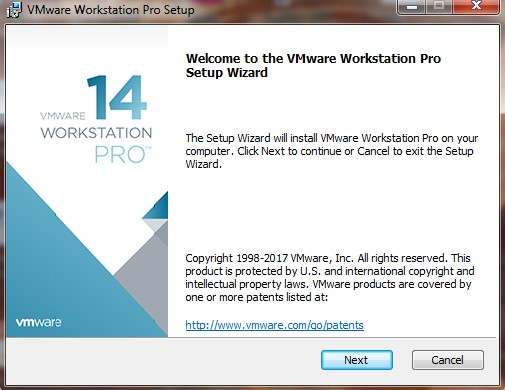
\includegraphics[width=10cm]{./Imagenes/WM01} 
	\end{center}

	\item Paso 02 :

	\begin{center}
	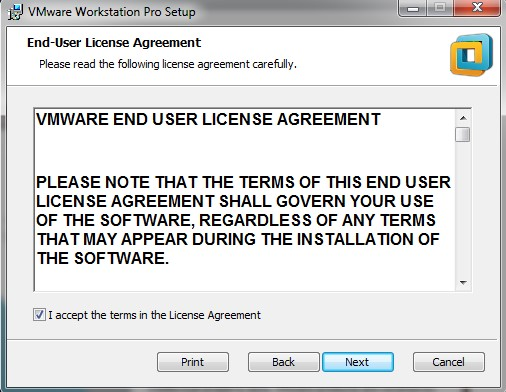
\includegraphics[width=10cm]{./Imagenes/WM02} 
	\end{center}

	\hfill \break
	\hfill \break
	\hfill \break
	\hfill \break
	\hfill \break
	\hfill \break
	\item Paso 03 :

	\begin{center}
	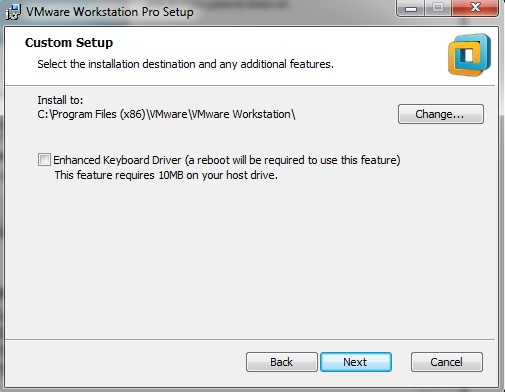
\includegraphics[width=10cm]{./Imagenes/WM03} 
	\end{center}

	\item Paso 04 :

	\begin{center}
	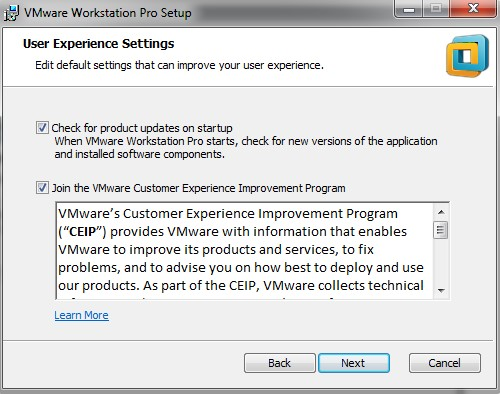
\includegraphics[width=10cm]{./Imagenes/WM04} 
	\end{center}

	\hfill \break
	\hfill \break
	\hfill \break
	\hfill \break
	\hfill \break
	\hfill \break
	\hfill \break
	\hfill \break
	\item Paso 05 : ahora ya instalamos el programa

	\begin{center}
	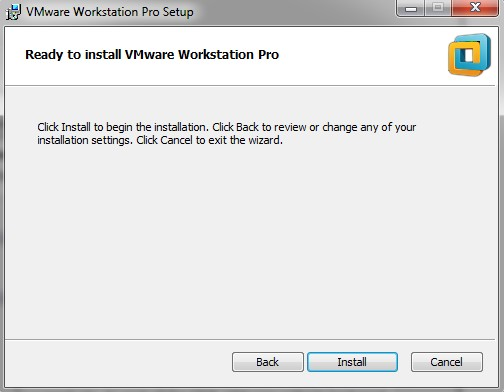
\includegraphics[width=10cm]{./Imagenes/WM05} 
	\end{center}

	\item Paso 06 :

	\begin{center}
	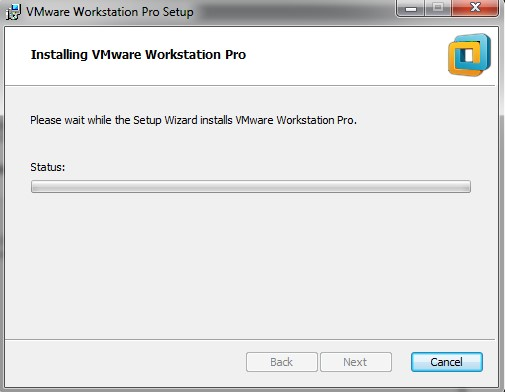
\includegraphics[width=10cm]{./Imagenes/WM06} 
	\end{center}

	\hfill \break
	\hfill \break
	\hfill \break
	\hfill \break
	\hfill \break
	\hfill \break
	\hfill \break
	\hfill \break
	\item Paso 07 :

	\begin{center}
	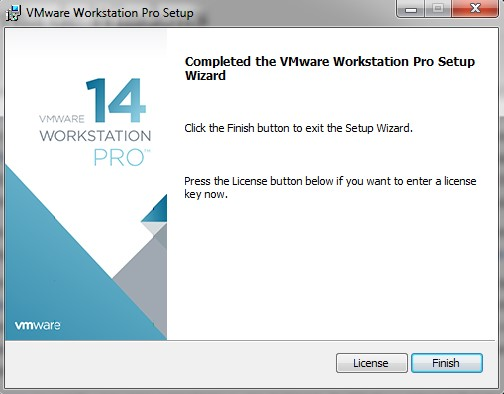
\includegraphics[width=10cm]{./Imagenes/WM07} 
	\end{center}

	\item Paso 08 : Ingresamos la clave del producto

	\begin{center}
	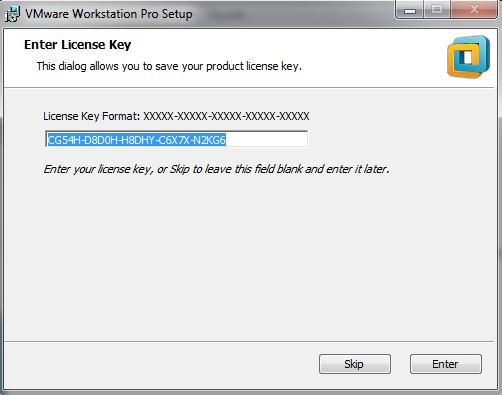
\includegraphics[width=10cm]{./Imagenes/WM08} 
	\end{center}

	\hfill \break
	\hfill \break
	\hfill \break
	\hfill \break
	\hfill \break
	\hfill \break
	\hfill \break
	\hfill \break
	\item Paso 09 :

	\begin{center}
	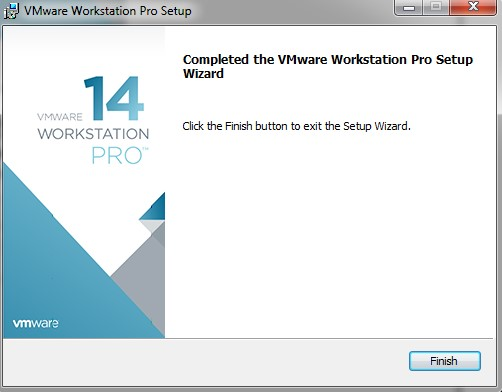
\includegraphics[width=10cm]{./Imagenes/WM09} 
	\end{center}

	\item Paso 10 : Listo

	\begin{center}
	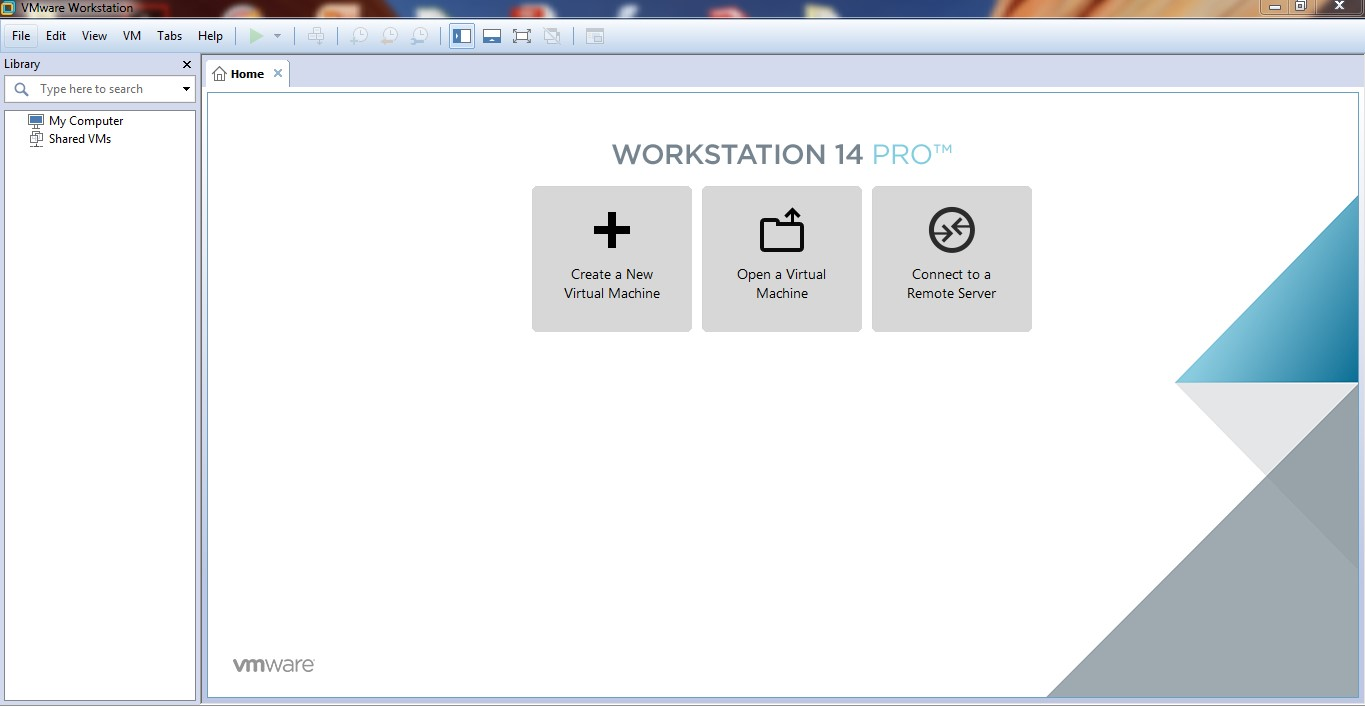
\includegraphics[width=10cm]{./Imagenes/WM10} 
	\end{center}
	
	

\end{enumerate} 
